\documentclass[11pt,a4paper]{article}

\usepackage[utf8]{inputenc}
\usepackage[T1]{fontenc}
\usepackage[margin=2.5cm]{geometry}
\usepackage{amsmath,amssymb,amsthm,bm}
\usepackage{booktabs,array}
\usepackage{enumitem}
\usepackage{tikz}
\usetikzlibrary{arrows.meta,calc,positioning}
\usepackage[most]{tcolorbox}
\usepackage[colorlinks=true,linkcolor=blue!50!black]{hyperref}

\setlength{\parskip}{0.5em}
\setlength{\parindent}{0pt}

% ---------- theorem-like environments (boxed) ----------
\theoremstyle{definition}
\newtheorem{definition}{Definition}[section]
\newtheorem{example}[definition]{Example}
\newtheorem{algorithm}[definition]{Algorithm}
\theoremstyle{plain}
\newtheorem{theorem}[definition]{Theorem}
\newtheorem{lemma}[definition]{Lemma}
\newtheorem{proposition}[definition]{Proposition}
\newtheorem{corollary}[definition]{Corollary}

\tcbset{thmbox/.style={enhanced,breakable,colback=gray!4,colframe=black!55,
  boxrule=0.6pt,arc=2pt,left=6pt,right=6pt,top=4pt,bottom=4pt,before skip=8pt,after skip=8pt}}
\tcolorboxenvironment{definition}{thmbox}
\tcolorboxenvironment{example}{thmbox}
\tcolorboxenvironment{algorithm}{thmbox}
\tcolorboxenvironment{theorem}{thmbox}
\tcolorboxenvironment{lemma}{thmbox}
\tcolorboxenvironment{proposition}{thmbox}
\tcolorboxenvironment{corollary}{thmbox}

\newtcolorbox{intuition}{enhanced,breakable,colback=blue!5,colframe=blue!65!black,
  coltitle=white,fonttitle=\bfseries,title=Intuition,boxrule=0.6pt,arc=2pt,
  left=6pt,right=6pt,top=4pt,bottom=4pt,before skip=8pt,after skip=10pt}

% ---------- shortcuts ----------
\newcommand{\R}{\mathbb{R}}
\newcommand{\qv}{\bm{q}}
\newcommand{\zv}{\bm{z}}
\newcommand{\wv}{\bm{w}}
\newcommand{\vv}{\bm{v}}
\DeclareMathOperator{\rank}{rank}
\DeclareMathOperator{\ad}{ad}

\title{\textbf{Autonomous and Mobile Robotics}\\[2pt]
\large Kinematic Models of Wheeled Mobile Robots II:\\ Bicycle-Equivalent Vehicles and Chained Forms}
\date{}

\begin{document}
\maketitle
\tableofcontents
\bigskip

% =====================================================================
\section{Vehicles Kinematically Equivalent to the Bicycle}
% =====================================================================

Several vehicles that look different share the same kinematic model as the bicycle:
the \emph{tricycle} (front-wheel or rear-wheel drive) and the \emph{car-like} robot.
In all of them the pair of front (steering) wheels can be replaced by a single
\emph{virtual} wheel placed at the midpoint between the two wheels, and the configuration is
\[
  \qv=\begin{pmatrix}x\\y\\\theta\\\phi\end{pmatrix},
\]
where $(x,y)$ is the position of the midpoint of the rear axle, $\theta$ the orientation of the body and $\phi$ the steering angle.
A \emph{differential-drive} robot has instead the same model as the unicycle, with the reference point centred on the axis of the driving wheels.

\begin{intuition}
Replacing two wheels by one is legitimate because of the \emph{instantaneous centre of rotation}:
at any instant a rigid body moves as if rotating about a single point (the CR), and pure rolling forces the motion of every wheel to be perpendicular to the line joining the wheel to that point. Whatever happens on the left and the right is therefore described by one ``average'' wheel on the vehicle's axis of symmetry.
\end{intuition}

\subsection{Ackermann steering}

Consider a car-like robot whose two front wheels are steered. Each wheel, rolling without slipping, cannot move along its axle, so its \emph{zero-motion line} is the line containing the axle. For the vehicle to move, all zero-motion lines must meet at one common point, the CR.

If the two front wheels were steered by the \emph{same} angle, they would be parallel: the two zero-motion lines would also be parallel, no common point could exist together with the rear-axle line, and the car would necessarily \emph{slip}.
The cure is the \textbf{Ackermann steering geometry}: the external front wheel is steered slightly \emph{less} than the internal one, so that the three axle lines meet in a single CR lying on the rear axle line. In practice this is obtained mechanically with a four-bar linkage (the steering trapezoid).

\begin{figure}[ht]
\centering
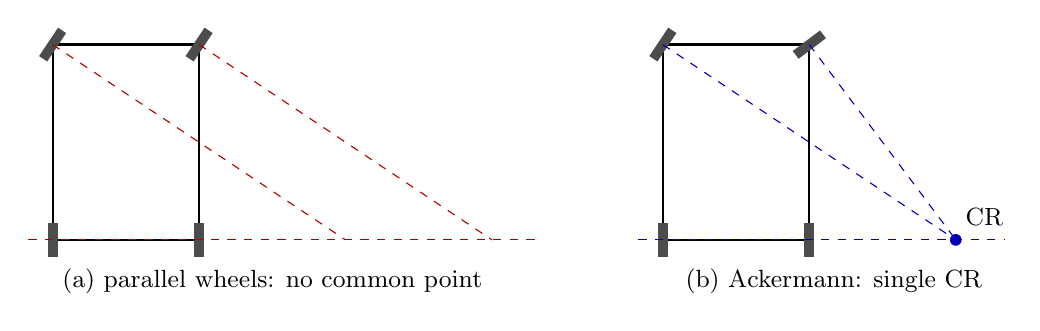
\begin{tikzpicture}[scale=0.62,>=Stealth]
% ---- panel (a): parallel wheels
\begin{scope}
  \draw[thick] (0,0) rectangle (3,4);
  \fill[black!70] (-0.1,-0.35) rectangle (0.1,0.35); \fill[black!70] (2.9,-0.35) rectangle (3.1,0.35);
  \begin{scope}[shift={(0,4)},rotate=-33.7]\fill[black!70] (-0.1,-0.35) rectangle (0.1,0.35);\end{scope}
  \begin{scope}[shift={(3,4)},rotate=-33.7]\fill[black!70] (-0.1,-0.35) rectangle (0.1,0.35);\end{scope}
  \draw[dashed,red!70!black] (-0.5,0)--(10,0);
  \draw[dashed,red!70!black] (0,4)--(6,0);
  \draw[dashed,red!70!black] (3,4)--(9,0);
  \node[below] at (4.5,-0.4) {\small (a) parallel wheels: no common point};
\end{scope}
% ---- panel (b): Ackermann
\begin{scope}[xshift=12.5cm]
  \draw[thick] (0,0) rectangle (3,4);
  \fill[black!70] (-0.1,-0.35) rectangle (0.1,0.35); \fill[black!70] (2.9,-0.35) rectangle (3.1,0.35);
  \begin{scope}[shift={(0,4)},rotate=-33.7]\fill[black!70] (-0.1,-0.35) rectangle (0.1,0.35);\end{scope}
  \begin{scope}[shift={(3,4)},rotate=-53.1]\fill[black!70] (-0.1,-0.35) rectangle (0.1,0.35);\end{scope}
  \draw[dashed,blue!70!black] (-0.5,0)--(7,0);
  \draw[dashed,blue!70!black] (0,4)--(6,0);
  \draw[dashed,blue!70!black] (3,4)--(6,0);
  \fill[blue!70!black] (6,0) circle (0.12);
  \node[above right] at (6,0.1) {\small CR};
  \node[below] at (3.5,-0.4) {\small (b) Ackermann: single CR};
\end{scope}
\end{tikzpicture}
\caption{Zero-motion lines of the wheels (dashed) of a car turning right. With parallel front wheels (a) they never meet in one point; with Ackermann steering (b) the outer (left) wheel is turned less than the inner one and everything converges in one CR.}
\end{figure}

\begin{intuition}
Think of the car going around a bend: the inner front wheel travels on a smaller circle than the outer one, so it must be turned \emph{more}. If both were turned equally, one of them would be fighting the other, dragging sideways on the road, and that is exactly the slipping that the kinematic model forbids.
\end{intuition}

% =====================================================================
\section{Chained Forms}
% =====================================================================

The kinematic models of many wheeled robots can be brought into a (rather) \emph{canonical} form, the chained form.

\begin{definition}[$(2,n)$ chained form]\label{def:chained}
A driftless system with two inputs and $n$ state variables is in \emph{$(2,n)$ chained form} if (the first number is the number of inputs, the second the number of coordinates)
\begin{align*}
  \dot z_1 &= w_1,\\
  \dot z_2 &= w_2,\\
  \dot z_3 &= z_2\,w_1,\\
  &\;\;\vdots\\
  \dot z_n &= z_{n-1}\,w_1 ,
\end{align*}
or, in vector form,
\[
  \dot{\zv}=\begin{pmatrix}1\\0\\z_2\\\vdots\\z_{n-1}\end{pmatrix}w_1+\begin{pmatrix}0\\1\\0\\\vdots\\0\end{pmatrix}w_2
  = \bm{\gamma}_1(\zv)\,w_1+\bm{\gamma}_2\,w_2 .
\]
\end{definition}

The structure is a \emph{cascade of integrators}: $w_1$ is integrated to give $z_1$; $w_2$ is integrated to give $z_2$; and every following variable is obtained by multiplying the previous one by $w_1$ and integrating.

\begin{figure}[ht]
\centering
\resizebox{\textwidth}{!}{%
\begin{tikzpicture}[>=Stealth,
  int/.style={draw,minimum width=0.9cm,minimum height=0.8cm},
  mul/.style={draw,circle,inner sep=1pt}]
  % row of w1
  \draw[->] (-0.2,2.6)--(1.4,2.6) node[pos=0,left] {$w_1$};
  \node[int] (i1) at (2,2.6) {$\int$};
  \draw[->] (i1)--(3.6,2.6) node[right] {$z_1$};
  \draw (0.7,2.6)--(0.7,1.4) -- (9,1.4);
  \fill (0.7,2.6) circle (1.5pt);
  % chain
  \draw[->] (-0.2,0)--(1.0,0) node[pos=0,left] {$w_2$};
  \node[int] (i2) at (1.5,0) {$\int$};
  \node[mul] (m3) at (3.6,0) {$\times$};
  \node[int] (i3) at (5,0) {$\int$};
  \node[mul] (m4) at (6.9,0) {$\times$};
  \node at (7.9,0) {$\cdots$};
  \node[mul] (mn) at (9,0) {$\times$};
  \node[int] (in) at (10.5,0) {$\int$};
  \draw[->] (i2)--(m3) node[pos=0.5,above] {$z_2$};
  \draw[->] (m3)--(i3);
  \draw[->] (i3)--(m4) node[pos=0.5,above] {$z_3$};
  \draw[->] (m4)--(7.4,0);
  \draw[->] (8.4,0)--(mn) node[pos=0.4,above] {$z_{n-1}$};
  \draw[->] (mn)--(in);
  \draw[->] (in)--(12,0) node[right] {$z_n$};
  \foreach \m in {m3,m4,mn} {\draw[->] (\m |- 0,1.4)--(\m);}
\end{tikzpicture}}
\caption{Block diagram of a $(2,n)$ chained form: the signal $w_1$ is distributed to all the multipliers.}
\end{figure}

\subsection{Controllability}

\begin{proposition}\label{prop:chainedctrl}
Every $(2,n)$ chained form is controllable: the accessibility distribution has dimension $\dim\Delta_A=n$ at every $\zv$.
\end{proposition}
\begin{proof}
With $\bm{\gamma}_2=\bm e_2$ constant, the Lie bracket is $[\bm\gamma_1,\bm\gamma_2]=\frac{\partial\bm\gamma_2}{\partial\zv}\bm\gamma_1-\frac{\partial\bm\gamma_1}{\partial\zv}\bm\gamma_2=-\frac{\partial\bm\gamma_1}{\partial\zv}\bm e_2=-\bm e_3$, because the only non-zero derivative of $\bm\gamma_1$ with respect to $z_2$ is that of its third entry. Repeating the same argument,
\[
 \ad^k_{\bm\gamma_1}\bm\gamma_2=(-1)^k\bm e_{k+2},\qquad k=0,\dots,n-2 .
\]
Hence $\bm\gamma_1,\bm\gamma_2,\ad_{\bm\gamma_1}\bm\gamma_2,\dots,\ad^{n-2}_{\bm\gamma_1}\bm\gamma_2$ are $n$ vectors that span $\R^n$ (from $\bm e_2,\dots,\bm e_n$ one gets $\bm e_1$ out of $\bm\gamma_1$), i.e.\ $\dim\Delta_A=n$. By Chow's theorem the system is controllable.
\end{proof}

\begin{intuition}
The two inputs directly move only $z_1$ and $z_2$. But $w_1$ ``feeds'' $z_3$ through $z_2$, $z_3$ feeds $z_4$, and so on: the effect of $w_2$ propagates \emph{down the chain} through the interplay with $w_1$. Each extra Lie bracket (an infinitesimal ``wiggle'': move along $\bm\gamma_1$, then $\bm\gamma_2$, then back) opens up exactly one new direction, and there are just enough of them to reach all $n$ coordinates.
\end{intuition}

\subsection{Why chained forms are useful}

\begin{proposition}[Linearity under constant input]\label{prop:linear}
If $w_1(t)\equiv c$ is constant, the chained form becomes a \emph{linear} time-invariant system in $(z_2,\dots,z_n)$ with input $w_2$ (and $z_1=ct+z_1(0)$). If $w_1$ is piecewise constant, the system is piecewise linear.
\end{proposition}
\begin{proof}
For $w_1=c$ the equations read $\dot z_1=c$, $\dot z_2=w_2$, $\dot z_i=c\,z_{i-1}$, $i=3,\dots,n$: all right-hand sides are linear in $(z_2,\dots,z_n,w_2)$.
\end{proof}

\begin{intuition}
The nonlinearity of the chained form is entirely due to the \emph{product} of a state with the input $w_1$. Freeze $w_1$ and the product becomes a plain gain. This is very handy in digital control, where inputs are held constant between sampling instants: within each sampling interval the system is linear, and one can use all of linear-systems theory.
\end{intuition}

\begin{proposition}[Transformability, fact]\label{prop:transform}
All controllable driftless systems with $n\le 4$ and $2$ inputs can be put in chained form (under standard regularity assumptions). This means there exist
\begin{itemize}[nosep]
  \item a \emph{coordinate transformation} $\zv=\bm\alpha(\qv)$ from the original coordinates $\qv$ to the chained-form coordinates, and
  \item an \emph{input transformation} $\wv=\bm\beta(\qv)\,\vv$, with $\bm\beta(\qv)$ invertible (so that $\vv$ are the original, linearly independent, inputs).
\end{itemize}
\end{proposition}

\begin{intuition}
The chained form is a change of ``language'': the robot is the same, but written in coordinates and with inputs that make its structure transparent. The transformations are built so that the system after the change is exactly a cascade of integrators.
\end{intuition}

% =====================================================================
\section{Chained Form of the Unicycle}
% =====================================================================

The unicycle kinematics
\[
 \dot x=v\cos\theta,\qquad \dot y=v\sin\theta,\qquad\dot\theta=\omega
\]
is a $(2,3)$ system: it should be mapped to $\dot z_1=w_1$, $\dot z_2=w_2$, $\dot z_3=z_2w_1$.

\begin{proposition}\label{prop:unicycle}
The coordinate and input transformations
\begin{align*}
 z_1&=\theta, & w_1&=\omega,\\
 z_2&=x\cos\theta+y\sin\theta, & w_2&=v-z_3\,\omega,\\
 z_3&=x\sin\theta-y\cos\theta,
\end{align*}
bring the unicycle into $(2,3)$ chained form.
\end{proposition}
\begin{proof}
Direct check. First $\dot z_1=\dot\theta=\omega=w_1$. Then
\begin{align*}
 \dot z_2&=\dot x\cos\theta-x\sin\theta\,\dot\theta+\dot y\sin\theta+y\cos\theta\,\dot\theta\\
 &=v(\cos^2\theta+\sin^2\theta)-(x\sin\theta-y\cos\theta)\dot\theta=v-z_3\,\omega=w_2,\\
 \dot z_3&=\dot x\sin\theta+x\cos\theta\,\dot\theta-\dot y\cos\theta+y\sin\theta\,\dot\theta\\
 &=v(\cos\theta\sin\theta-\sin\theta\cos\theta)+(x\cos\theta+y\sin\theta)\dot\theta=z_2\,\omega=z_2\,w_1 .
\end{align*}
The map is invertible: $x=z_2\cos z_1+z_3\sin z_1$, $y=z_2\sin z_1-z_3\cos z_1$.
\end{proof}

\begin{figure}[ht]
\centering
\begin{tikzpicture}[>=Stealth,scale=1.1]
  % global frame
  \draw[->] (-0.5,0)--(5,0) node[right] {$x$};
  \draw[->] (0,-1.6)--(0,3) node[above] {$y$};
  % rotated axes
  \draw[->,thick,blue!70!black] (0,0)--(4.1,2.87) node[above right] {$z_2$};
  \draw[->,thick,red!70!black] (0,0)--(1.44,-2.05) node[below right] {$z_3$};
  \draw (0.8,0) arc (0:35:0.8); \node at (1.15,0.3) {$\theta$};
  % robot
  \begin{scope}[shift={(3.2,1)},rotate=35]
    \fill[black!75] (-0.25,-0.1) rectangle (0.25,0.1);
    \draw[->,thick] (0.25,0)--(0.85,0);
  \end{scope}
  \node[right] at (3.3,0.75) {$(x,y)$};
  % projections
  \draw[dashed] (3.2,1)--(2.613,1.831);
  \draw[dashed] (3.2,1)--(0.585,-0.835);
  \fill (2.613,1.831) circle (1.2pt); \fill (0.585,-0.835) circle (1.2pt);
\end{tikzpicture}
\caption{Meaning of the chained coordinates of the unicycle: $z_2$ and $z_3$ are the components of the position $(x,y)$ along the axis $z_2$ (the direction of heading $\theta$) and along the perpendicular axis $z_3$ obtained by rotating it by $-90^\circ$; $z_1=\theta$.}
\end{figure}

\begin{intuition}
The new coordinates are simply the robot's position \emph{expressed in a frame rotated by the heading angle}. Rotating the robot ($w_1=\omega$) changes the frame, and thereby changes $z_2$ and $z_3$: the position in the rotating frame changes even if the robot does not translate, which is the origin of the product term $z_2\,w_1$. The input $w_2=v-z_3\omega$ is the forward speed corrected by this frame-rotation effect.
\end{intuition}

% =====================================================================
\section{Chained Form of the Bicycle}
% =====================================================================

The bicycle (equivalently the car-like robot) has $n=4$ coordinates and is therefore a $(2,4)$ system:
\[
 \dot z_1=w_1,\quad \dot z_2=w_2,\quad\dot z_3=z_2w_1,\quad\dot z_4=z_3w_1 .
\]

\begin{proposition}\label{prop:bicycle}
For the rear-wheel drive car with model $\dot x=v\cos\theta$, $\dot y=v\sin\theta$, $\dot\theta=\tfrac{v}{\ell}\tan\phi$, $\dot\phi=\omega$, in the region $|\theta|<\pi/2$ the transformation
\[
 z_1=x,\quad z_2=\frac{\tan\phi}{\ell\cos^3\theta},\quad z_3=\tan\theta,\quad z_4=y,
 \qquad w_1=v\cos\theta,\quad w_2=\dot z_2
\]
gives the $(2,4)$ chained form.
\end{proposition}
\begin{proof}
$\dot z_1=v\cos\theta=w_1$ and $\dot z_2=w_2$ by definition (explicitly, $w_2=\dfrac{\omega}{\ell\cos^3\theta\cos^2\phi}+\dfrac{3\sin\theta\tan^2\phi}{\ell^2\cos^4\theta}\,v$, invertible with respect to $\omega$). Next
\[
 \dot z_3=\frac{\dot\theta}{\cos^2\theta}=\frac{v\tan\phi}{\ell\cos^2\theta}=v\cos\theta\cdot\frac{\tan\phi}{\ell\cos^3\theta}=z_2w_1,
\qquad
 \dot z_4=v\sin\theta=v\cos\theta\tan\theta=z_3w_1 .\qedhere
\]
\end{proof}

\begin{intuition}
Here $z_1$ and $z_4$ are the Cartesian coordinates, $z_3$ is (the tangent of) the heading, and $z_2$ is (a scaled version of) the curvature of the path. The chain reads: speed along $x$ drives the slope of the path; the slope drives $y$; and the steering rate changes the curvature. It is the familiar picture of ``curvature $\to$ heading $\to$ position'' written as a cascade.
\end{intuition}

% =====================================================================
\section{Adding Trailers}
% =====================================================================

Consider adding one (or more) \textbf{trailers} to the unicycle or to the bicycle. The new vehicle is \emph{still transformable to chained form}, as long as each trailer is \emph{hinged at the midpoint between the two wheels} of the preceding body (the axle midpoint of the car or of the previous trailer).

\begin{intuition}
Hitching at the axle midpoint keeps the geometry ``rolling-friendly'': each trailer wheel is again the point of a body that can only move along its own heading direction, exactly like the rear wheel of the car. The new body therefore adds one new coordinate (its angle $\theta_t$) and one new link in the chain, rather than breaking the structure. A fully worked example (a tricycle with a trailer, with its constraints and kinematic model) is given in Section~\ref{sec:test}.
\end{intuition}
% =====================================================================
\section{Class Test 2009 -- Problem 1: Tricycle with a Trailer}\label{sec:test}
% =====================================================================

\begin{example}[Problem 1]
Consider the mobile robot obtained by attaching a trailer to a rear-wheel drive tricycle. The trailer is a rigid body with an axle carrying two fixed wheels, and is connected to the midpoint of the tricycle rear axle through a revolute joint. Both two-wheel axles can be assimilated to a single wheel located at the midpoint of the axle.
\begin{enumerate}[nosep]
 \item Find a set of generalized coordinates for the robot, and clearly indicate them on the drawing.
 \item Write the Pfaffian kinematic constraints to which the robot is subject.
 \item Derive a kinematic model of the system.
\end{enumerate}
\end{example}

\subsection{Generalized coordinates}

A convenient choice is
\[
 \qv=(x\;\;y\;\;\theta\;\;\phi\;\;\theta_t)^T,
\]
i.e.\ the generalized coordinates of the tricycle plus one additional coordinate for the trailer. Here $(x,y)$ is the midpoint $P$ of the rear axle, $\theta$ the heading of the tricycle, $\phi$ the steering angle of the front wheel, and $\theta_t$ the orientation of the trailer; $P_f$ is the centre of the front wheel (at distance $\ell$ from $P$) and $P_t$ the midpoint of the trailer axle (at distance $\ell_t$ from $P$). The robot has three wheels: the tricycle front wheel, the tricycle rear wheel and the trailer wheel.

\begin{figure}[ht]
\centering
\begin{tikzpicture}[>=Stealth,scale=1.15]
  \draw[->] (-0.2,0)--(8,0) node[right] {$x$};
  \draw[->] (-0.2,0)--(-0.2,4.6) node[above] {$y$};
  % points
  \coordinate (P) at (4,2);
  \coordinate (Pf) at (6.27,3.06);
  \coordinate (Pt) at (2.03,1.65);
  % body and hitch
  \draw[thick] (Pt)--(P)--(Pf);
  % wheels
  \begin{scope}[shift={(4,2)},rotate=25] \fill[black!75] (-0.08,-0.4) rectangle (0.08,0.4); \end{scope}
  \begin{scope}[shift={(6.27,3.06)},rotate=55] \fill[black!75] (-0.3,-0.08) rectangle (0.3,0.08); \end{scope}
  \begin{scope}[shift={(2.03,1.65)},rotate=10] \fill[black!75] (-0.08,-0.4) rectangle (0.08,0.4); \end{scope}
  \fill (P) circle (1.5pt) (Pf) circle (1.5pt) (Pt) circle (1.5pt);
  \node[above left] at (P) {$P$};
  \node[above right] at (Pf) {$P_f$};
  \node[below left] at (Pt) {$P_t$};
  \node at (3.15,2.15) {$\ell_t$};
  \node at (5.2,2.75) {$\ell$};
  % angles
  \draw[dotted] (P)--++(1.8,0);
  \draw ($(P)+(1.1,0)$) arc (0:25:1.1); \node at (5.35,2.25) {$\theta$};
  \draw[dotted] (Pf)--++(1.2,0);
  \draw[dotted] (Pf)--++(25:1.2);
  \draw ($(Pf)+(0.9,0.38)$) arc (25:55:0.9); \node at (7.3,3.5) {$\phi$};
  \draw[dotted] (Pt)--++(1.0,0);
  \draw ($(Pt)+(0.8,0)$) arc (0:10:0.8); \node at (3.1,1.8) {};
  \node at (3.0,1.55) {\small $\theta_t$};
  % projections for x, y
  \draw[dotted] (P)--(4,0); \node[below] at (4,0) {$x$};
  \draw[dotted] (P)--(-0.2,2); \node[left] at (-0.2,2) {$y$};
\end{tikzpicture}
\caption{Tricycle with trailer. Generalized coordinates $\qv=(x,y,\theta,\phi,\theta_t)$.}
\end{figure}

\subsection{Pfaffian kinematic constraints}

There are three kinematic constraints (one pure-rolling condition per wheel):
\begin{align*}
 \dot x_f\sin(\theta+\phi)-\dot y_f\cos(\theta+\phi)&=0,\\
 \dot x\sin\theta-\dot y\cos\theta&=0,\\
 \dot x_t\sin\theta_t-\dot y_t\cos\theta_t&=0,
\end{align*}
where $(x_f,y_f)$ and $(x_t,y_t)$ are the Cartesian coordinates of $P_f$ and $P_t$:
\[
 x_f=x+\ell\cos\theta,\quad y_f=y+\ell\sin\theta,\qquad
 x_t=x-\ell_t\cos\theta_t,\quad y_t=y-\ell_t\sin\theta_t .
\]
Differentiating and substituting (for instance $\dot x_f=\dot x-\ell\dot\theta\sin\theta$, $\dot y_f=\dot y+\ell\dot\theta\cos\theta$, and the identities $\sin\theta\sin(\theta+\phi)+\cos\theta\cos(\theta+\phi)=\cos\phi$ and $\sin^2\theta_t+\cos^2\theta_t=1$) one obtains
\begin{align*}
 \dot x\sin(\theta+\phi)-\dot y\cos(\theta+\phi)-\dot\theta\,\ell\cos\phi&=0,\\
 \dot x\sin\theta-\dot y\cos\theta&=0,\\
 \dot x\sin\theta_t-\dot y\cos\theta_t+\ell_t\dot\theta_t&=0,
\end{align*}
or, in Pfaffian form $A^T(\qv)\dot{\qv}=0$,
\[
 \begin{pmatrix}
  \sin\theta&-\cos\theta&0&0&0\\
  \sin(\theta+\phi)&-\cos(\theta+\phi)&-\ell\cos\phi&0&0\\
  \sin\theta_t&-\cos\theta_t&0&0&\ell_t
 \end{pmatrix}
 \begin{pmatrix}\dot x\\\dot y\\\dot\theta\\\dot\phi\\\dot\theta_t\end{pmatrix}=0 .
\]

\begin{intuition}
Each wheel contributes one equation of the form ``velocity of the wheel centre $\perp$ axle direction'' (no lateral slipping). The first two rows (rear and front wheel of the tricycle) are the constraints of the bicycle; the third row is new and says that the trailer wheel is, again, forced to move along the direction of the trailer.
\end{intuition}

\subsection{Kinematic model}

Note that the submatrix made of the first two rows and the first four columns of $A^T$ coincides with the constraint matrix of the bicycle. A basis of the null space of $A^T$ can then be written by ``completing'' the basis found for the bicycle (in particular the rear-wheel drive version, since the tricycle has rear-wheel drive) with a suitable fifth entry:
\[
 G(\qv)=\begin{pmatrix}\bm g_1&\bm g_2\end{pmatrix}=
 \begin{pmatrix}
  \cos\theta&0\\ \sin\theta&0\\ \tan\phi/\ell&0\\0&1\\ -\sin(\theta_t-\theta)/\ell_t&0
 \end{pmatrix}.
\]
The kinematic control system is
\[
 \dot{\qv}=\bm g_1(\qv)\,v+\bm g_2(\qv)\,\omega ,
\]
where $v$ and $\omega$ are respectively the driving velocity and the steering velocity of the tricycle.

\emph{Check.} The third constraint applied to $\bm g_1$ gives $\cos\theta\sin\theta_t-\sin\theta\cos\theta_t+\ell_t\cdot\frac{-\sin(\theta_t-\theta)}{\ell_t}=\sin(\theta_t-\theta)-\sin(\theta_t-\theta)=0$, and the other two rows vanish exactly as in the bicycle.

\begin{intuition}
The driving input $v$ moves the tricycle exactly as in the bicycle and, in addition, \emph{pulls} the trailer: $\dot\theta_t$ is proportional to $\sin(\theta-\theta_t)$, so the trailer tends to align behind the tricycle when it moves forward (the further it is from alignment, the faster it rotates, and it stops rotating when aligned). The steering input $\omega$ only changes $\phi$ and leaves the others untouched.
\end{intuition}

\textbf{A different choice of coordinates.} The model depends on the chosen $\qv$; a different choice leads to an equivalent model via a change of coordinates. For example with $\qv'=(x\;y\;\theta\;\phi\;\delta)^T$, $\delta=\theta-\theta_t$, one has $\dot{\qv}'=\bm g_1'(\qv')v+\bm g_2'(\qv')\omega$ with
\[
 G'(\qv')=\begin{pmatrix}
  \cos\theta&0\\ \sin\theta&0\\ \tan\phi/\ell&0\\0&1\\ \tan\phi/\ell-\sin\delta/\ell_t&0
 \end{pmatrix},
\]
since $\dot\delta=\dot\theta-\dot\theta_t=v\big(\tan\phi/\ell-\sin\delta/\ell_t\big)$.

% =====================================================================
\section{Worked Exercise: A Rolling Wheel on the Plane}
% =====================================================================

\textbf{Setting.} A unicycle (a disk of radius $R$) moves on a plane. Extend the configuration vector by including the \emph{wheel (rolling) angle} $\phi$. We want to: (1) define the configuration space; (2) write the constraints; (3) show controllability; (4) describe a sequential manoeuvre.

\subsection{Configuration space and kinematic model}

The configuration is
\[
 \qv=\begin{pmatrix}x\\y\\\theta\\\phi\end{pmatrix}\in\R^2\times SO(2)\times SO(2),\qquad \dim=4 ,
\]
($\theta$ is the heading, $\phi$ the angle of rotation of the wheel about its horizontal axis). The unicycle equations $\dot x=v\cos\theta$, $\dot y=v\sin\theta$, $\dot\theta=\omega$ are completed by $\dot\phi=\omega_\phi$, where $\omega_\phi$ is the angular velocity of the wheel about its horizontal axis. Since the wheel rolls, $v=R\,\omega_\phi$, so
\[
 \begin{pmatrix}\dot x\\\dot y\\\dot\theta\\\dot\phi\end{pmatrix}
 =\begin{pmatrix}R\cos\theta\\R\sin\theta\\0\\1\end{pmatrix}\omega_\phi
 +\begin{pmatrix}0\\0\\1\\0\end{pmatrix}\omega .
\]

\subsection{Constraints}

Two pure-rolling conditions act on the wheel:
\begin{align*}
 \dot x\sin\theta-\dot y\cos\theta&=0 &&\text{(rolling laterally: no side slip, along the axle)},\\
 v=R\,\omega_\phi &&&\text{(rolling along the sagittal axis)}.
\end{align*}
Kinematically, the second one reads $\pm\sqrt{\dot x^2+\dot y^2}-R\dot\phi=0$, which is \emph{not} Pfaffian (it is not linear in $\dot{\qv}$).

\textbf{How to solve this.} Use $v=R\dot\phi$ and $v(\cos^2\theta+\sin^2\theta)=\dot x\cos\theta+\dot y\sin\theta$ to obtain
\[
 \dot x\cos\theta+\dot y\sin\theta-R\dot\phi=0 ,
\]
which \emph{is} Pfaffian. The constraint matrix is
\[
 A^T(\qv)=\begin{pmatrix}\sin\theta&-\cos\theta&0&0\\ \cos\theta&\sin\theta&0&-R\end{pmatrix},
\]
the first row being the lateral rolling condition and the second the rolling condition along the sagittal axis. The null space of $A^T(\qv)$ gives the same kinematic model as before, $\dot{\qv}=\bm g_1\omega_\phi+\bm g_2\omega$ with
\[
 \bm g_1=\begin{pmatrix}R\cos\theta\\R\sin\theta\\0\\1\end{pmatrix},\qquad
 \bm g_2=\begin{pmatrix}0\\0\\1\\0\end{pmatrix}.
\]

\begin{intuition}
The ``physical'' rolling condition is a statement about \emph{speeds}: the distance covered on the ground equals the radius times the angle turned. A speed contains a square root of the velocity components, which is not linear. The trick is to project the velocity on the heading direction, $\dot x\cos\theta+\dot y\sin\theta$, which is the signed forward speed, and which \emph{is} linear in $\dot{\qv}$. This keeps the sign (forward/backward) and brings the problem back to the Pfaffian world.
\end{intuition}

\subsection{Controllability}

\begin{proposition}\label{prop:rollwheel}
The rolling wheel on the plane is controllable (the accessibility distribution has dimension $4$ everywhere).
\end{proposition}
\begin{proof}
Compute the Lie brackets with $[\bm g_i,\bm g_j]=\frac{\partial\bm g_j}{\partial\qv}\bm g_i-\frac{\partial\bm g_i}{\partial\qv}\bm g_j$. Since $\bm g_2$ is constant,
\[
 \bm g_3:=[\bm g_1,\bm g_2]=-\frac{\partial\bm g_1}{\partial\qv}\bm g_2
 =-\begin{pmatrix}0&0&-R\sin\theta&0\\0&0&R\cos\theta&0\\0&0&0&0\\0&0&0&0\end{pmatrix}
 \begin{pmatrix}0\\0\\1\\0\end{pmatrix}=\begin{pmatrix}R\sin\theta\\-R\cos\theta\\0\\0\end{pmatrix}.
\]
This is linearly independent of $\bm g_1,\bm g_2$, so already $3$ directions are available. Further brackets:
\[
 [\bm g_1,\bm g_3]=\bm 0,\qquad [\bm g_2,\bm g_3]=\frac{\partial\bm g_3}{\partial\theta}=\begin{pmatrix}R\cos\theta\\R\sin\theta\\0\\0\end{pmatrix}=:\bm g_4 .
\]
Finally, the matrix $\begin{pmatrix}\bm g_1&\bm g_2&\bm g_3&\bm g_4\end{pmatrix}$ has the structure (reordering rows and columns, a block triangular matrix) in which only the $2\times2$ blocks on the diagonal matter. Its determinant is
\[
 \det\begin{pmatrix}R\cos\theta&0&R\sin\theta&R\cos\theta\\R\sin\theta&0&-R\cos\theta&R\sin\theta\\0&1&0&0\\1&0&0&0\end{pmatrix}=-R^2\neq0 .
\]
So $\rank\{\bm g_1,\bm g_2,\bm g_3,\bm g_4\}=4$ and by Chow's theorem the system is controllable.
\end{proof}

\begin{intuition}
Four coordinates, two inputs. Rolling forward and turning generate the sideways motion $\bm g_3$ (the parking manoeuvre: roll, turn, roll back, turn back); and turning the wheel's heading while a sideways displacement is present generates a further direction $\bm g_4$. Crucially, $\phi$ can only change when the wheel \emph{moves} (rolling), which is why all four directions need the brackets and not only the two inputs.
\end{intuition}

\subsection{A sequential manoeuvre}

\begin{algorithm}[Reaching a desired $(x_g,y_g,\theta_g,\phi_g)$]\label{alg:rollwheel}
Let the initial configuration be $(x_s,y_s,\theta_s,\phi_s)$.
\begin{enumerate}[nosep]
 \item Steps $1$--$3$ are as for the unicycle: drive the position and heading to the goal values, $x\to x_g$, $y\to y_g$, $\theta\to\theta_g$. At the end of this phase the wheel angle $\phi$ has some value which, in general, differs from $\phi_g$.
 \item Perform a \emph{circular motion} that brings $\phi$ to $\phi_g$ and leaves the robot in the same position and orientation. The wheel rolls along a circle of radius $r$ once around, so the rolled distance $2\pi r$ equals the arc length corresponding to the required change of the wheel angle:
 \[
   2\pi r=R\,(\phi_g-\phi_s),
 \]
 where $r$ is the radius of the circle and $R$ is the wheel radius ($\phi_s$ denotes the wheel angle at the start of this last phase).
\end{enumerate}
\end{algorithm}

\begin{figure}[ht]
\centering
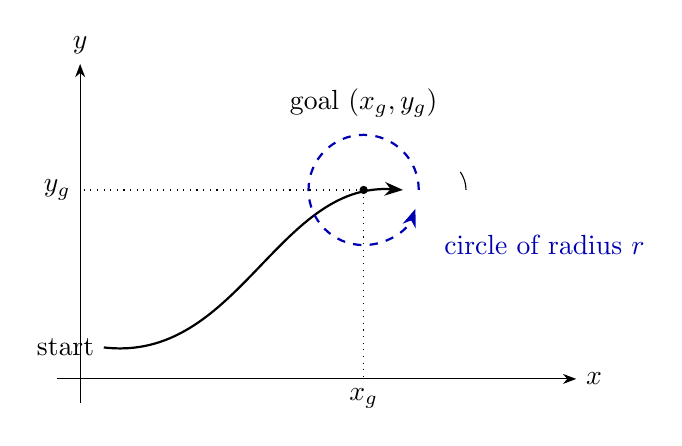
\begin{tikzpicture}[>=Stealth,scale=1.0]
  \draw[->] (-0.3,0)--(6.3,0) node[right] {$x$};
  \draw[->] (0,-0.3)--(0,4) node[above] {$y$};
  \draw[thick,->] (0.3,0.4) .. controls (2,0.2) and (2.5,2.5) .. (4.1,2.4);
  \node[left] at (0.3,0.4) {start};
  \draw[dashed,thick,blue!70!black,->] (4.3,2.4) arc (0:340:0.7);
  \fill (3.6,2.4) circle (1.5pt);
  \node[above] at (3.6,3.2) {goal $(x_g,y_g)$};
  \draw[dotted] (3.6,2.4)--(3.6,0); \draw[dotted] (3.6,2.4)--(0,2.4);
  \node[below] at (3.6,0) {$x_g$}; \node[left] at (0,2.4) {$y_g$};
  \node[blue!70!black,right] at (4.5,1.7) {circle of radius $r$};
  \draw (4.9,2.4) arc (0:35:0.4); 
\end{tikzpicture}
\caption{Sequential manoeuvre: first the unicycle-like motion to the goal position and heading (solid), then a circular motion at the goal (dashed) that only changes $\phi$.}
\end{figure}

\begin{intuition}
The wheel angle $\phi$ is only changed by rolling, but rolling also moves the robot. The trick is to roll \emph{in a closed loop}: after one full circle the robot is back at the same position and (modulo $2\pi$) the same heading, while the wheel has turned by an amount proportional to the length of the circle. Choosing $r$ gives exactly the missing wheel rotation. Systematic ways to do this will be seen in the next lecture, when we discuss planning.
\end{intuition}


% =====================================================================
\section{Summary}
% =====================================================================

\begin{center}
\small
\renewcommand{\arraystretch}{1.25}
\begin{tabular}{p{2.9cm}cccp{4.6cm}}
\toprule
\textbf{System} & $n$ & \textbf{Constraints} & \textbf{Controllable} & \textbf{Chained form}\\
\midrule
Unicycle / differential drive & 3 & 1 & yes & $(2,3)$ via $z_1=\theta$, $z_2=x\cos\theta+y\sin\theta$, $z_3=x\sin\theta-y\cos\theta$\\
Bicycle, tricycle, car-like (rear-wheel drive) & 4 & 2 & yes & $(2,4)$ via $z_1=x$, $z_2=\frac{\tan\phi}{\ell\cos^3\theta}$, $z_3=\tan\theta$, $z_4=y$ ($|\theta|<\pi/2$)\\
Tricycle with trailer (hinged at the axle midpoint) & 5 & 3 & yes & still transformable to chained form\\
Rolling wheel on the plane (with $\phi$) & 4 & 2 (after linearization of rolling) & yes (brackets $\bm g_3,\bm g_4$) & reached with a sequential manoeuvre\\
\bottomrule
\end{tabular}
\end{center}

\textbf{Key take-aways.}
\begin{itemize}
 \item Bicycle, tricycle and car-like robots share the same kinematic model; an Ackermann steering geometry (outer front wheel turned less than the inner one) guarantees a single CR and therefore pure rolling.
 \item The $(2,n)$ chained form $\dot z_1=w_1$, $\dot z_2=w_2$, $\dot z_i=z_{i-1}w_1$ is a cascade of integrators that is always controllable (via the Lie brackets $\ad^k_{\bm\gamma_1}\bm\gamma_2\propto\bm e_{k+2}$).
 \item With $w_1$ constant (or piecewise constant, as with digital control) the chained form is linear (piecewise linear), which makes control design easy.
 \item Unicycle and bicycle are put in chained form through a coordinate transformation $\zv=\bm\alpha(\qv)$ and an input transformation $\wv=\bm\beta(\qv)\vv$; adding trailers hinged at the axle midpoint preserves transformability.
 \item Constraints that are not Pfaffian at first sight (rolling of the wheel with $\phi$) can be made Pfaffian by projecting the velocity on the heading direction; controllability then follows from the Lie algebra rank condition and non-trivial configurations are reached by sequential manoeuvres.
\end{itemize}

\end{document}